\documentclass[a4paper, 14pt]{extarticle}

% Includes 
\usepackage[utf8]{inputenc} % UTF-8 encode
\usepackage[english, russian]{babel}
\usepackage{geometry} % adjust page layout 
\usepackage{graphicx} 
\usepackage{placeins} 
\usepackage{hyperref} 
\usepackage{amsmath} % math formulas 
\usepackage{setspace} % for set line spacing 
\usepackage{indentfirst} % indent on a first line after the paragraph 
% \usepackage{pgfplots} % for plots 
\usepackage{listings} % for code listings 
\usepackage{xcolor} % colors (used for listings)
\usepackage{sourcecodepro} % for another monospaced font 
\usepackage{cmap} % for correct search in pdf
\usepackage{afterpage,fancyhdr}

% debug
% \usepackage{showframe} % frame borders for demonstration 


%%% Custom commands
% commands for unnumbered sections
\newcommand{\usection}[1]{\section*{#1} \addcontentsline{toc}{section}{\protect\numberline{}#1}}
\newcommand{\usubsection}[1]{\subsection*{#1} \addcontentsline{toc}{subsection}{\protect\numberline{}#1}}
\newcommand{\usubsubsection}[1]{\subsubsection*{#1} \addcontentsline{toc}{subsubsection}{\protect\numberline{}#1}}


% Redefinition of section and subsection numbering style
\def\thesection{\arabic{section}.}
\def\thesubsection{\arabic{section}.\arabic{subsection}.}
\def\thesubsubsection{\arabic{section}.\arabic{subsection}.\arabic{subsubsection}.}



% Settings for links 
\hypersetup{
    colorlinks,
    citecolor=black,
    filecolor=black,
    linkcolor=black,
    urlcolor=black
}


% Layout
\geometry{
	left=30mm,
	top=20mm,
	right=15mm,
	bottom=20mm,
	marginparsep=0mm,
	marginparwidth=0mm,
	headheight=16pt,
	headsep=5mm, 
}

\linespread{1.5} % line spacing
\setlength{\parskip}{\baselineskip}  % Add space between paragraphs

% overfull hbox settings
\tolerance 10000 % default 200, max 10000
\hbadness 10000 % default 1000, max 10000
\emergencystretch 0pt  % default 0pt, how much the lines can stretch for the sake of good line breaks
\hfuzz 0.4pt % ignore overfull box less than 
\widowpenalty=10000 % no lines at the start of the page
\vfuzz \hfuzz % don't care about underfull vbox if overfull is acceptable
\raggedbottom % if the page is not filled, align the content to the bottom


% Redefinition of table of contents command to get centered heading
\makeatletter
\renewcommand\tableofcontents{ 
  \begin{singlespace}
    \null\hfill\textbf{\Large\contentsname}\hfill\null\par
    \@mkboth{\MakeUppercase\contentsname}{\MakeUppercase\contentsname}%
    \@starttoc{toc}
  \end{singlespace}
}
\makeatother

\pagestyle{fancy}
\fancypagestyle{style}{ % создание нового стиля style
	\fancyhf{} % очистка колонтитулов
	% \fancyhead[LO, RE]{} % название документа наверху
	\fancyhead[RO, LE]{\rightmark} % название section наверху
	\renewcommand{\headrulewidth}{0.25pt} % толщина линии сверху
	\renewcommand{\footrulewidth}{0pt} % толцина линии снизу
}
\fancypagestyle{plain}{ % создание нового стиля plain -- полностью пустого
	\fancyhf{}
	\renewcommand{\headrulewidth}{0pt}
}


% Listings settings
\definecolor{codegreen}{rgb}{0, 0.6, 0}
\definecolor{codegray}{rgb}{0.5, 0.5, 0.5}
\definecolor{codepurple}{rgb}{0.58, 0, 0.82}
\definecolor{backcolour_gray}{rgb}{0.98, 0.98, 0.98}

\lstdefinestyle{python_white}{
  language=Python,
  backgroundcolor=\color{backcolour_gray},   
  commentstyle=\color{codegreen},
  keywordstyle=\color{blue},
  numberstyle=\tiny\color{codegray},
  stringstyle=\color{codepurple},
  basicstyle=\ttfamily\small\singlespacing,
  breakatwhitespace=true,         
  breaklines=true,                 
  captionpos=b, % t/b                  
  keepspaces=true,                 
  numbers=none, % none/left/right                    
  numbersep=5pt,                  
  showspaces=false,                
  showstringspaces=false,
  showtabs=false,                  
  tabsize=2,
  frame=single, % none/leftline/topline/bottomline/lines/single/shadowbox
  rulecolor=\color{gray}, % frame color 
}


\lstset{style=python_white}


% For title page
\def\name{Отчет по лабораторной работе №6} 
\def\subname{<<Обработка изображений>>}
\def\madeby{Братушка Н. И.}
\def\teacher{Перегудин А. А., \\
Пашенко А. В.}

\begin{document}

% Title page 
\begin{titlepage}

\thispagestyle{empty}

\title{

НИУ ИТМО 
\vspace{2em}

\begin{center}
\LARGE{\textbf{\name}}

\subname

\end{center}

\vfill

\begin{flushright}
\large{ 
Выполнил: \textbf{\madeby} \\
Группа: \textbf{R3238} \\
Поток:  \textbf{ЧМ 1.4} \\
Преподаватель: \textbf{\teacher} 
}
\end{flushright}	

\vfill


\includegraphics[width=5cm]{images/ITMO_logo.png} 

\begin{center}
\normalsize{Санкт-Петербург, \the\year}
\end{center}
}

\date{}
\maketitle
\thispagestyle{empty}
\end{titlepage} % Title page

\thispagestyle{plain}
\addtocounter{page}{1} % Inc counter to start from 2 
\tableofcontents % Table of contents
\section{Фильтрация изображений}
В первом задании займёмся фильтрацией изоображения под номером 8, приведенного ниже:
\vspace{1cm}
\begin{figure}[ht!]
    \centering
    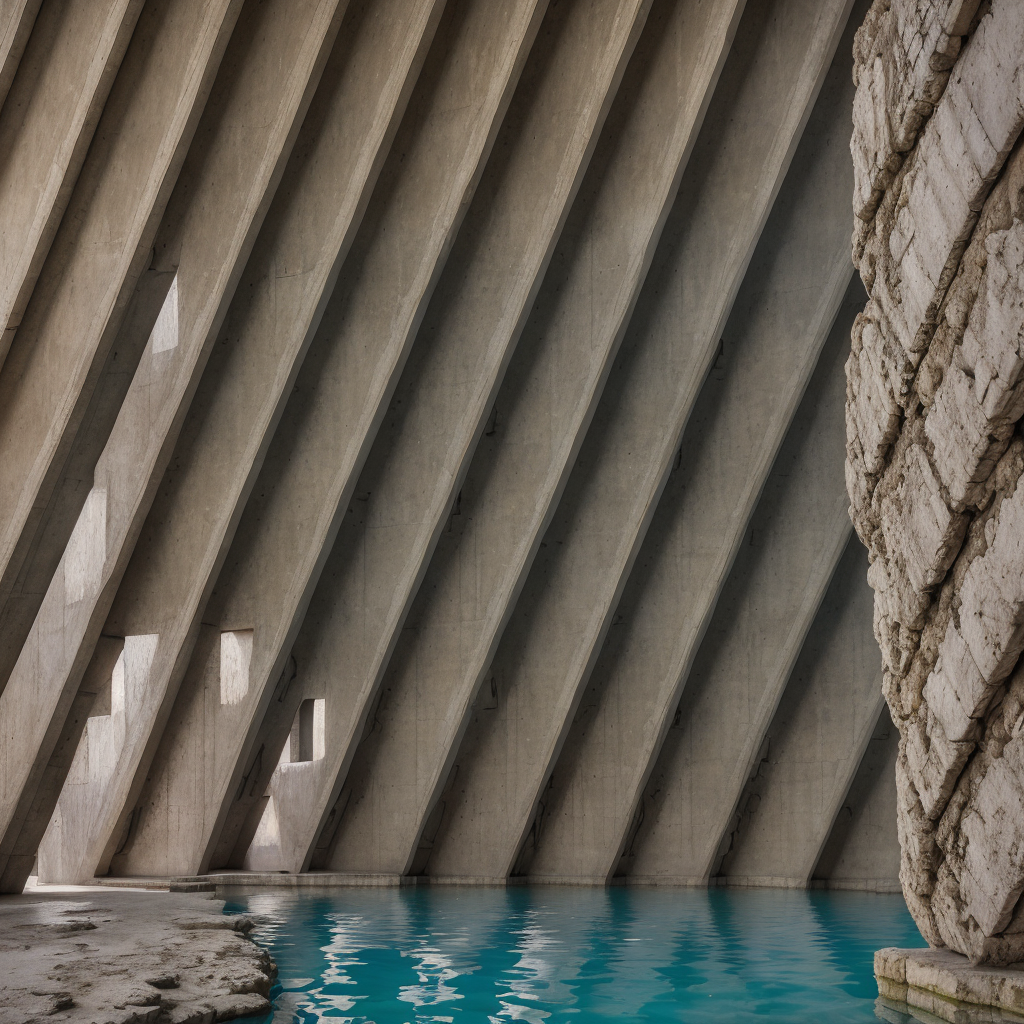
\includegraphics[width=0.95\textwidth]{images/source_images/task_1/8.png}
    \caption{Изображение 8 -- Бэтпещера нормального человека}
    \label{fig:photo_8}
\end{figure}
\clearpage
Найдём логарифм модуля сдвинутого Фурье-образа:
\vspace{1.5cm}
\begin{figure}[ht!]
    \centering
    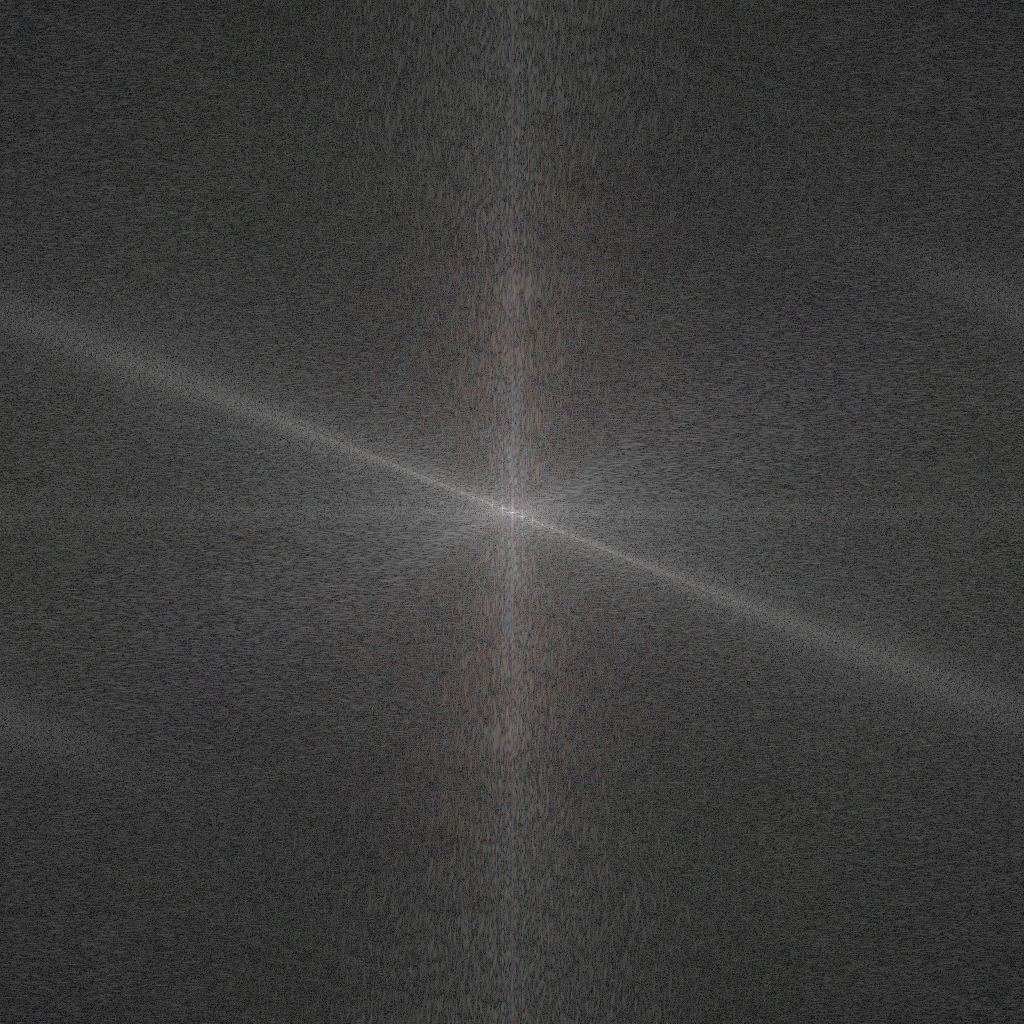
\includegraphics[width=0.95\textwidth]{images/result/task_1/Fourier_8.png}
    \caption{Логарифм модуля сдвинутого Фурье-образа}
    \label{fig:image_8}
\end{figure}
\vspace{1cm}

Помимо центрального пика, на изображении отчётливо видны 8 пиков.
\clearpage
\begin{figure}[ht!]
    \centering
    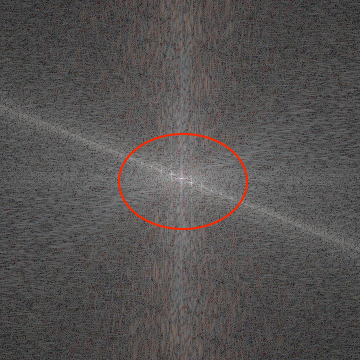
\includegraphics[width=0.6\textwidth]{images/result/task_1/Fourier_8_peaks.png}
    \caption{Цветовые пики, соответствующие гармоникам}
    \label{fig:image_8_peaks}
\end{figure}

Будем последовательно закрашивать каждую пару пиков. Начнём с самой яркой пары:

\begin{figure}[ht!]
    \centering
    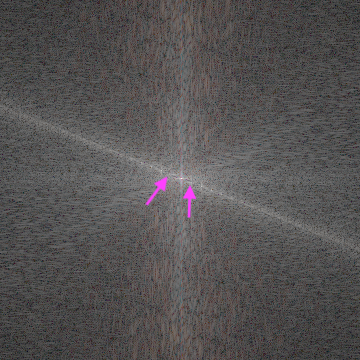
\includegraphics[width=0.6\textwidth]{images/result/task_1/Fourier_8_modified_1_peaks.png}
    \caption{Образ Фурье после удаления двух пиков}
    \label{fig:image_8_m1}
\end{figure}

\vspace{2cm}

\begin{figure}[ht!]
    \centering
    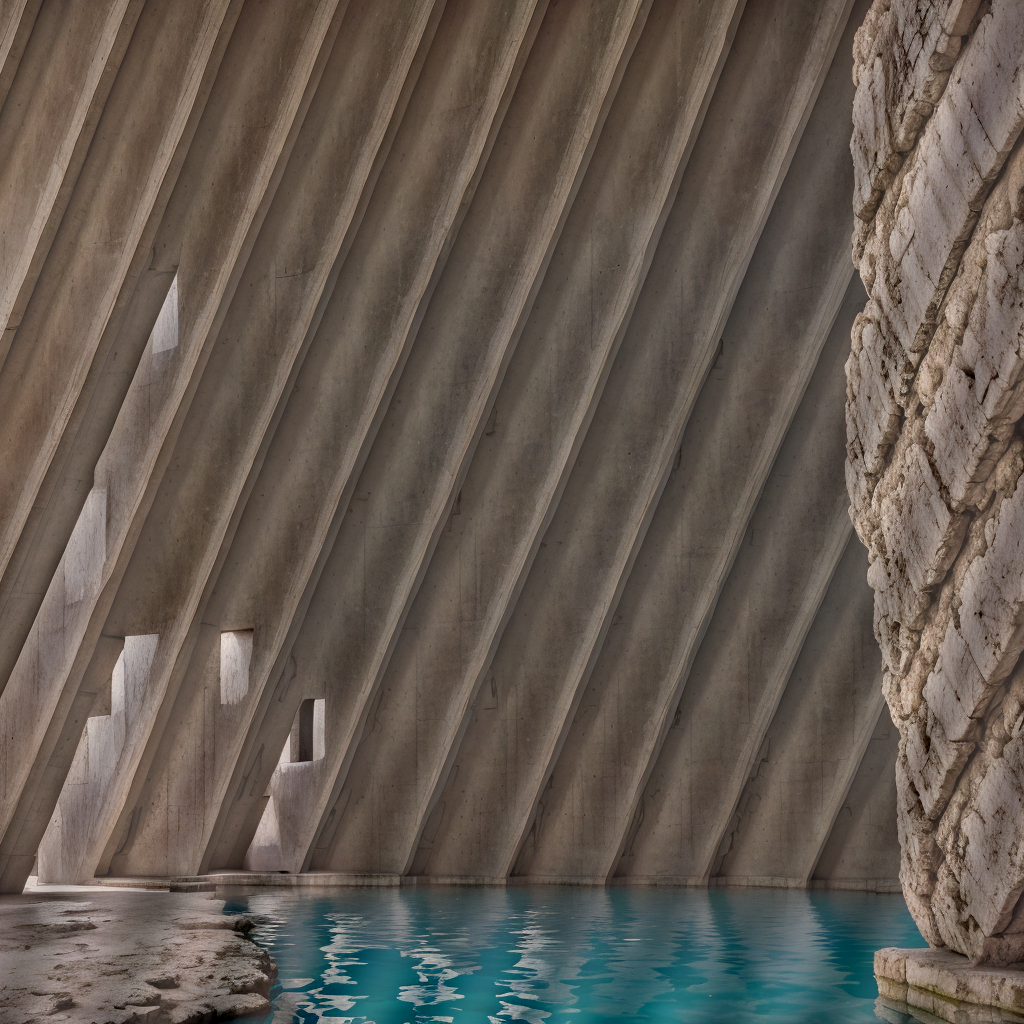
\includegraphics[width=0.95\textwidth]{images/result/task_1/result_8_1.png}
    \caption{Изображение после удаления двух пиков}
    \label{fig:photo_8_m1}
\end{figure}

Изображение стало более блеклым, на нём появились темно-серые полосы, особенно это заметно на бетонных столбах и скалах. При этом темные участки (пространство между столбами). Это связано с тем, что светлые пики на образе были закрашены серыми пикселями (рис. \ref{fig:image_8_m1}).

Теперь закрасим следующую пару пиков:


\begin{figure}[ht!]
    \centering
    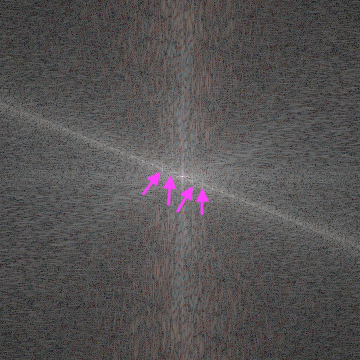
\includegraphics[width=\textwidth]{images/result/task_1/Fourier_8_modified_2_peaks.png}
    \caption{Образ Фурье после удаления четырех пиков}
    \label{fig:image_8_m2}
\end{figure}
\clearpage
\begin{figure}[ht!]
    \centering
    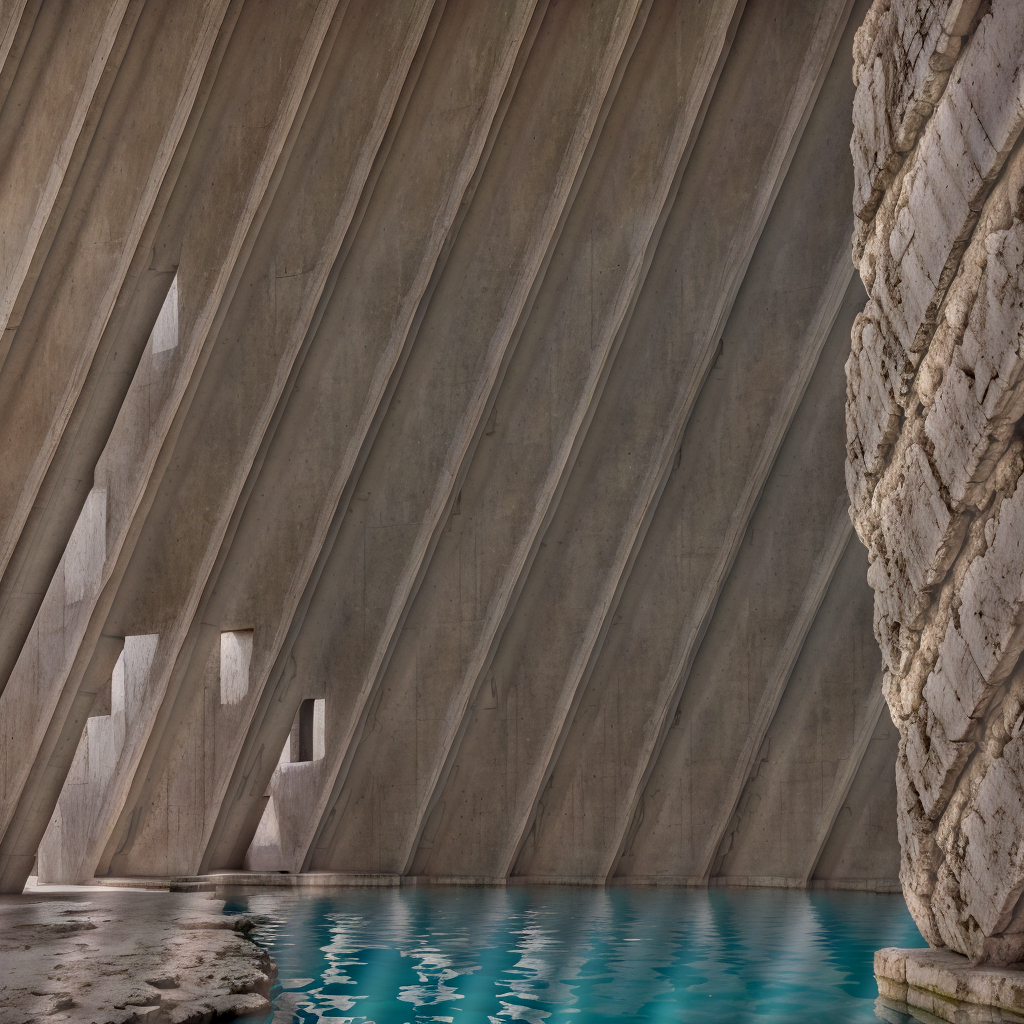
\includegraphics[width=0.95\textwidth]{images/result/task_1/result_8_2.png}
    \caption{Изображение после удаления четырех пиков}
    \label{fig:photo_8_m2}
\end{figure}

Полосы на изображении стали шире и более блеклыми, темные области между столбами -- светлее. 

Далее закрасим все пики на Фурье-образе:

\begin{figure}[ht!]
    \centering
    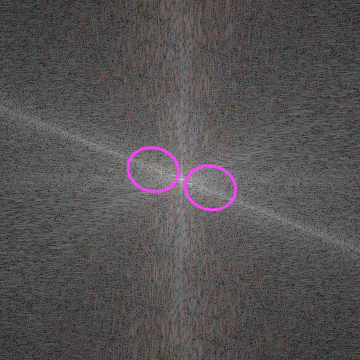
\includegraphics[width=\textwidth]{images/result/task_1/Fourier_8_modified_3_peaks.png}
    \caption{Образ Фурье после удаления восьми пиков}
    \label{fig:image_8_m3}
\end{figure}
\clearpage
\begin{figure}[ht!]
    \centering
    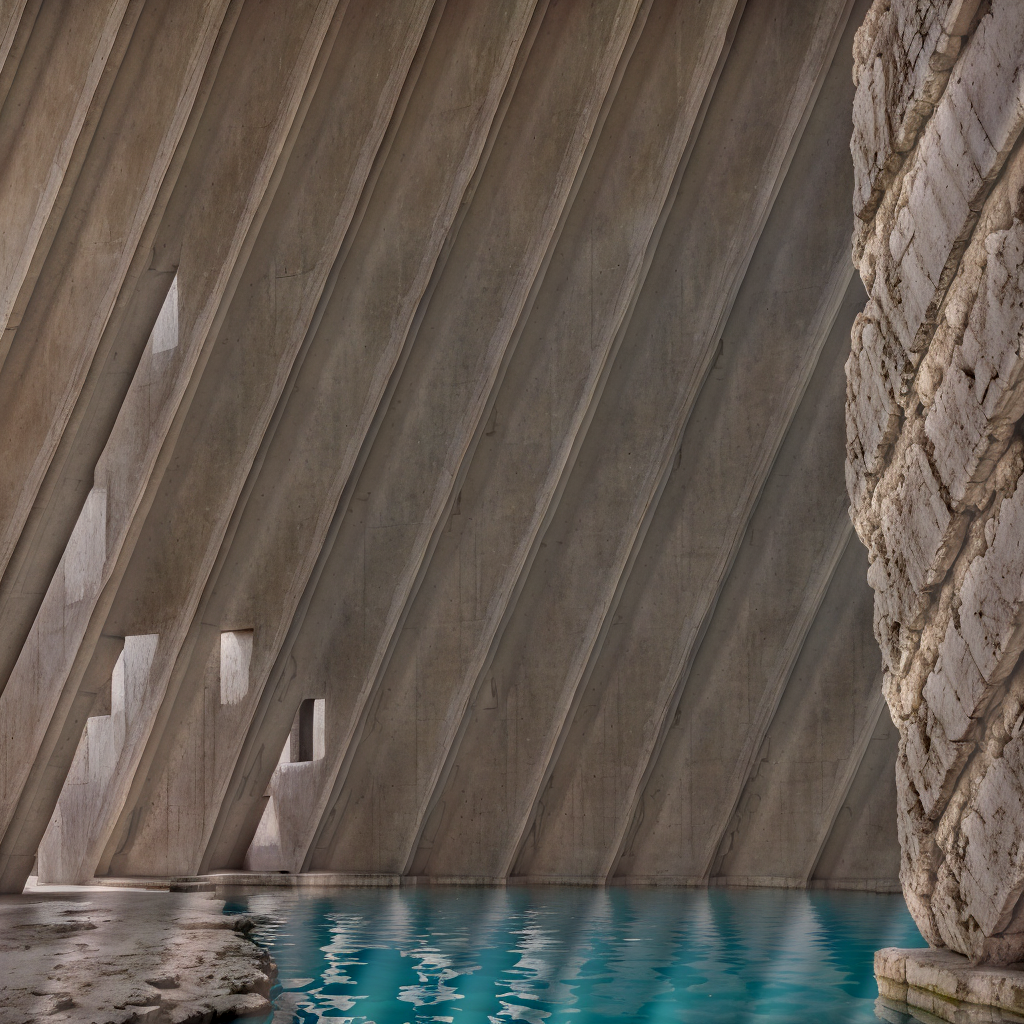
\includegraphics[width=0.95\textwidth]{images/result/task_1/result_8_3.png}
    \caption{Изображение после удаления восьми пиков}
    \label{fig:photo_8_m3}
\end{figure}
Полученное изображение стало менее контрастным по сравнению с предыдущими. 

Обращаясь к исходному изображению (рис. \ref{fig:photo_8}), полученные фотографии выглядят менее красочными и объёмными: бетонные столбы <<слиплись>>, став одной стеной. В целом полученные изображения выглядят неестественно: на поверхности воды появились темные полосы, на скале темные и светлые области поменялись местами.

\FloatBarrier

\section{Размытие и резкость}
 Для следующих двух заданий будем использовать следующее изображение:

 \begin{figure}[ht!]
    \centering
    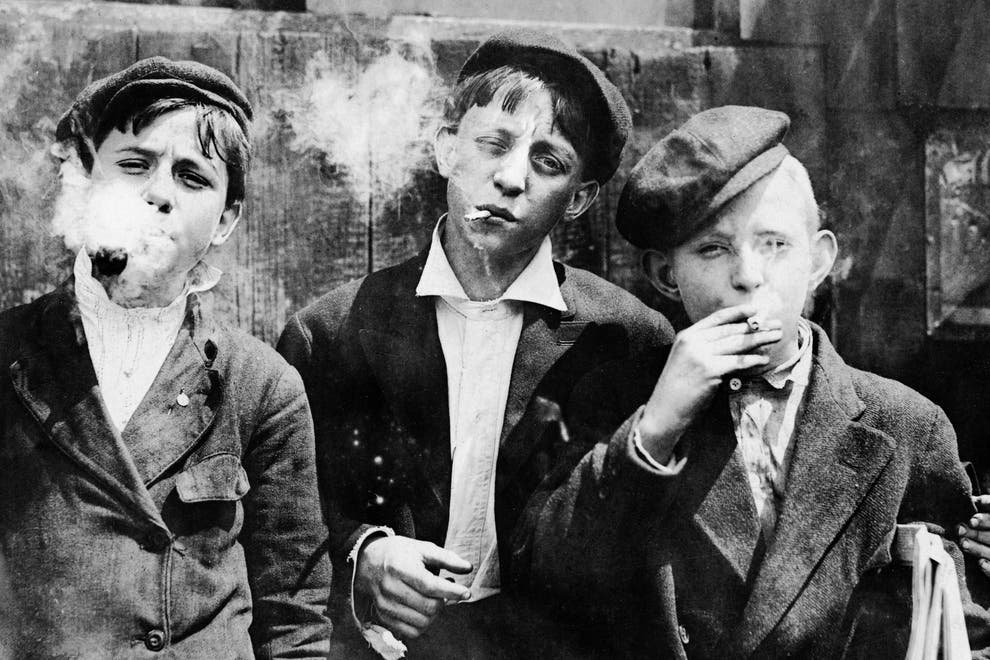
\includegraphics[width=0.95\textwidth]{images/source_images/task_2_3/smoking-boys.jpg}
    \caption{Lewis Hine -- 11:00 A.M. Monday, May 9th, 1910. Newsies at Skeeter's Branch, Jefferson near Franklin. They were all smoking. Location- St. Louis, Missouri}
    \label{fig:smoking_boys}
\end{figure}

 \subsection{Размытие изображения}
 \subsubsection{Блочное размытие}

 Для выполнения блочного размытия необходимо использовать квадратную матрицу $N \times N$, элементами которой являются дроби $\frac{1}{N}$. Рассмотрим и сравним блочное размытие при $N=5, 9, 11$ при помощи свертки и перемножения Фурье-образов с последующим обратным преобразованием.

 \begin{figure}[ht!]
    \centering
    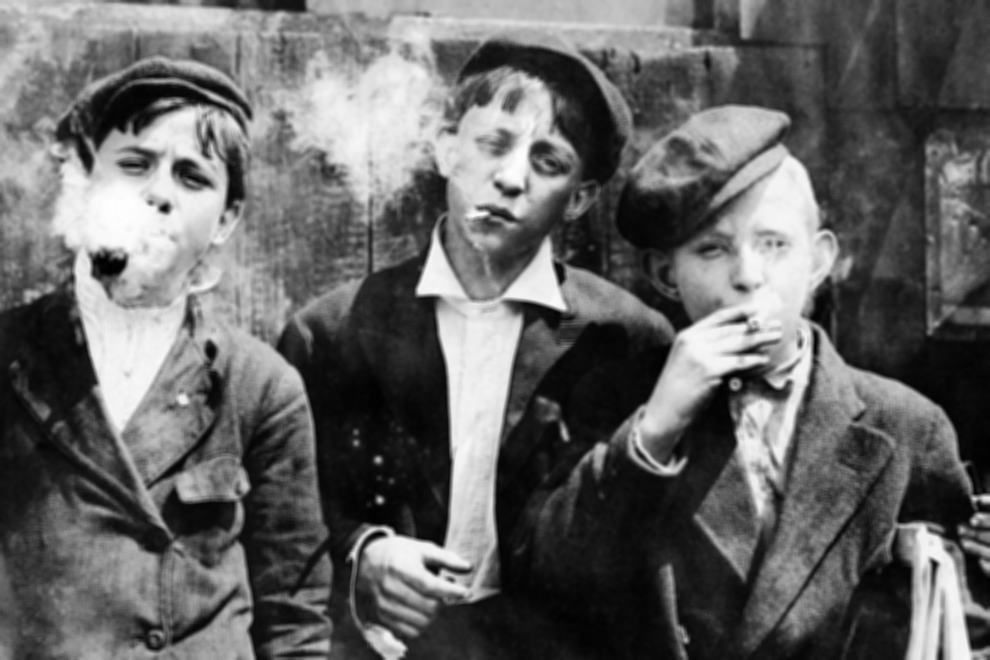
\includegraphics[width=0.95\textwidth]{images/result/task_2/Averaging_5.png}
    \caption{Результат блочного размытия при помощи свертки при $N=5$}
    \label{fig:av_c_5}
\end{figure}

\begin{figure}[ht!]
    \centering
    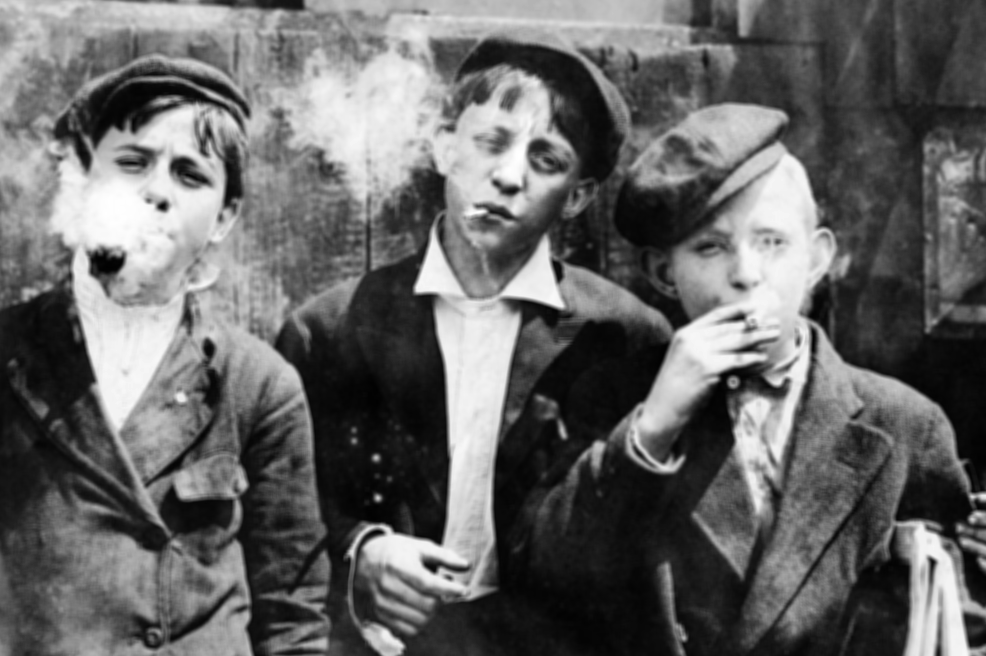
\includegraphics[width=0.95\textwidth]{images/result/task_2/Averaging_fourier_5.png}
    \caption{Результат блочного размытия при помощи преобразований Фурье при $N=5$}
    \label{fig:av_f_5}
\end{figure}

\begin{figure}[ht!]
    \centering
    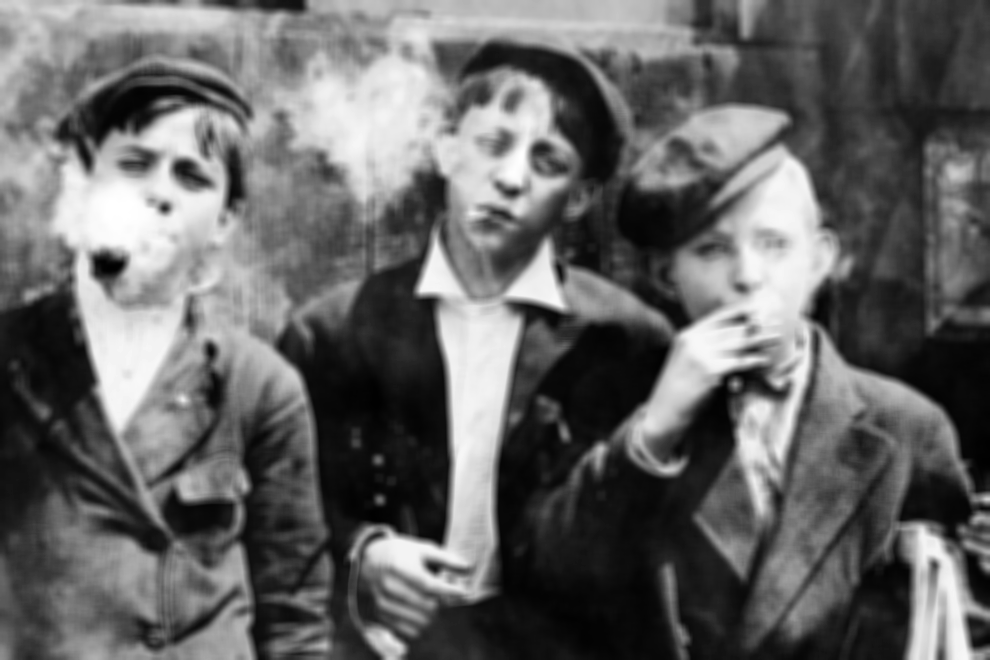
\includegraphics[width=0.95\textwidth]{images/result/task_2/Averaging_9.png}
    \caption{Результат блочного размытия при помощи свертки при $N=9$}
    \label{fig:av_c_9}
\end{figure}

\begin{figure}[ht!]
    \centering
    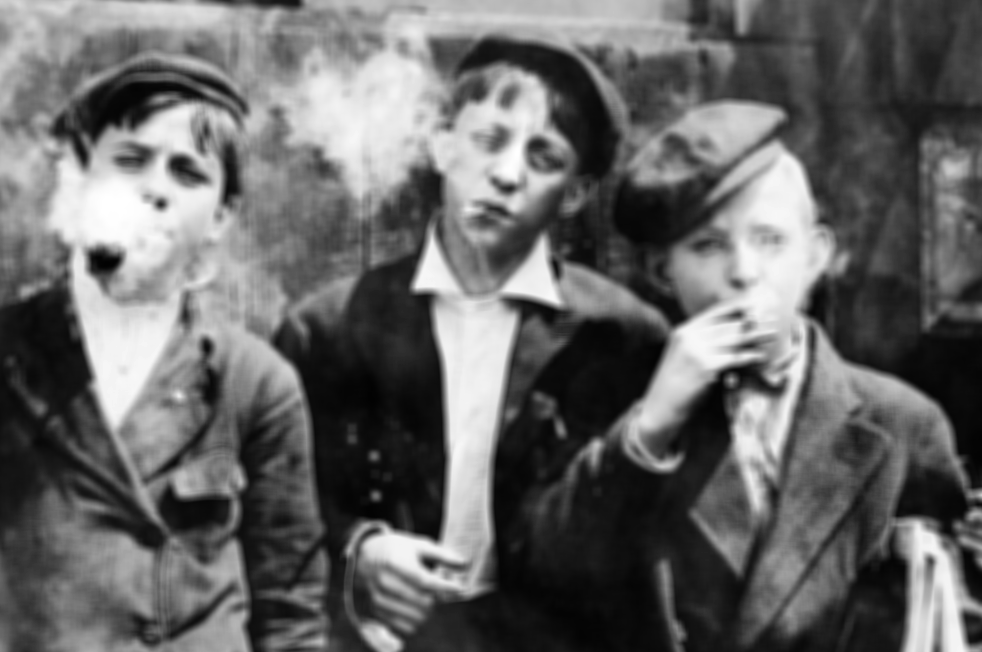
\includegraphics[width=0.95\textwidth]{images/result/task_2/Averaging_fourier_9.png}
    \caption{Результат блочного размытия при помощи преобразований Фурье при $N=9$}
    \label{fig:av_f_9}
\end{figure}

\begin{figure}[ht!]
    \centering
    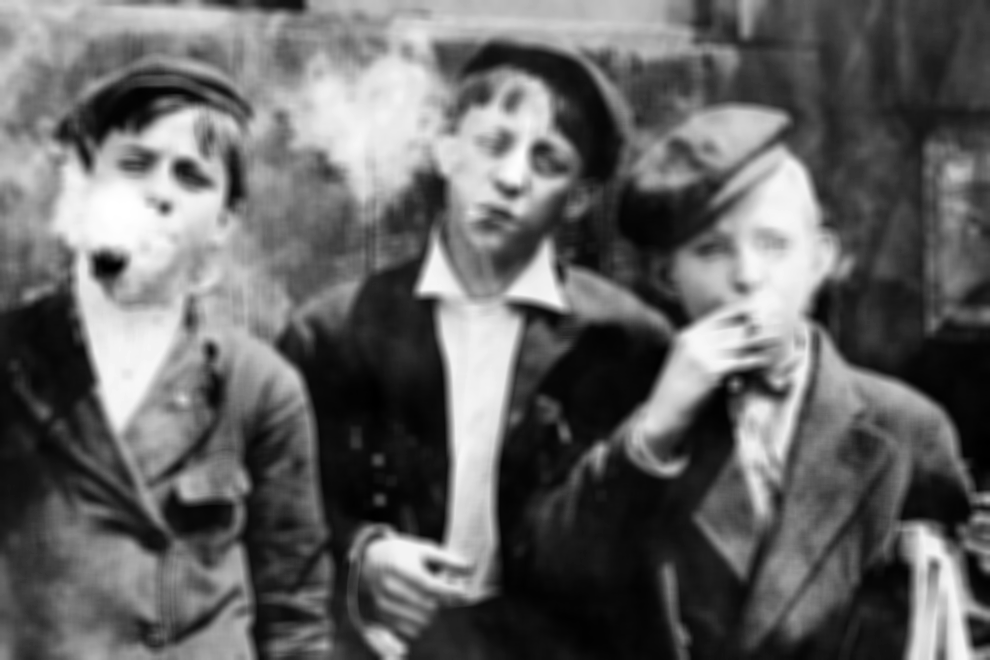
\includegraphics[width=0.95\textwidth]{images/result/task_2/Averaging_11.png}
    \caption{Результат блочного размытия при помощи свертки при $N=11$}
    \label{fig:av_c_11}
\end{figure}

\begin{figure}[ht!]
    \centering
    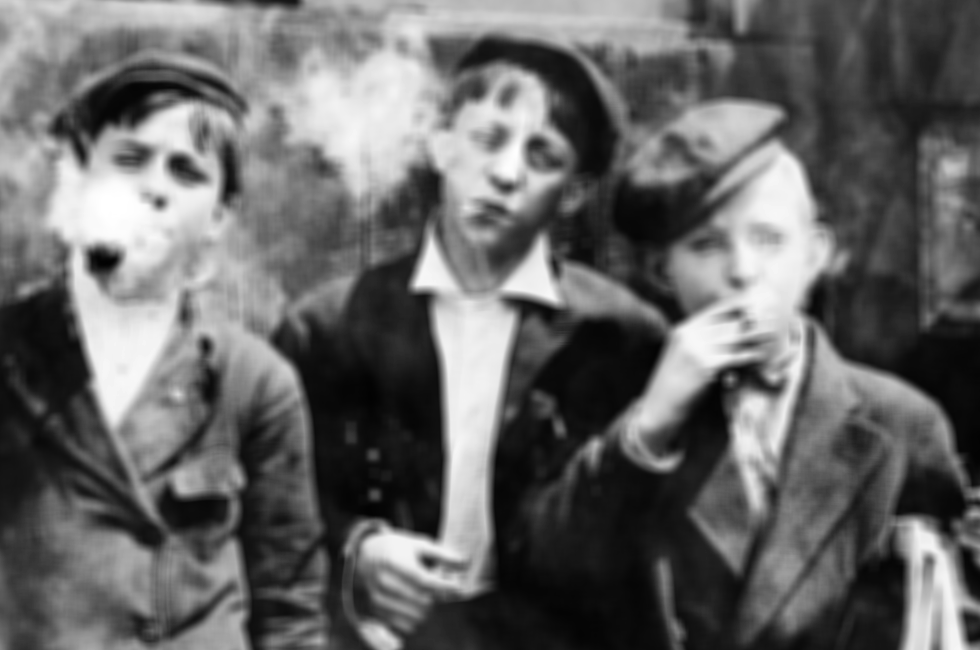
\includegraphics[width=0.95\textwidth]{images/result/task_2/Averaging_fourier_11.png}
    \caption{Результат блосного размытия при помощи преобразований Фурье при $N=11$}
    \label{fig:av_f_11}
\end{figure}
Полученные результаты идентичны, что подтверждает эквивалентность свертки и произведения Фурье-образов.
\clearpage
\subsubsection{Гауссово размытие}

Переходим к размытию по Гауссу при $N=5, 9, 11$:
\begin{figure}[ht!]
    \centering
    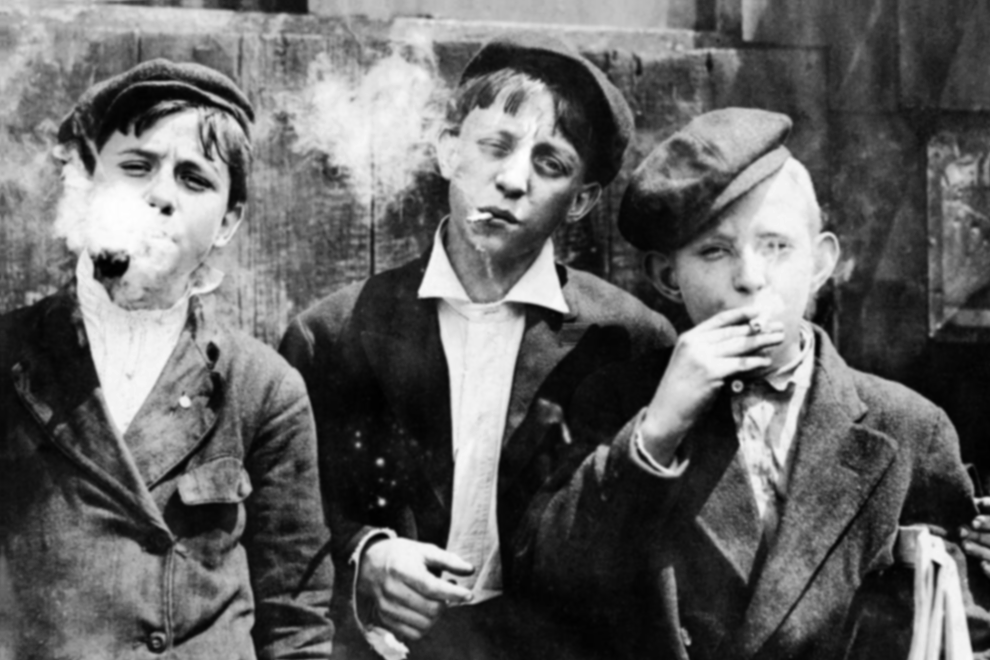
\includegraphics[width=0.85\textwidth]{images/result/task_2/Gaussian_5.png}
    \caption{Результат размытия по Гауссу при помощи свертки при $N=5$}
    \label{fig:ga_c_5}
\end{figure}

\begin{figure}[ht!]
    \centering
    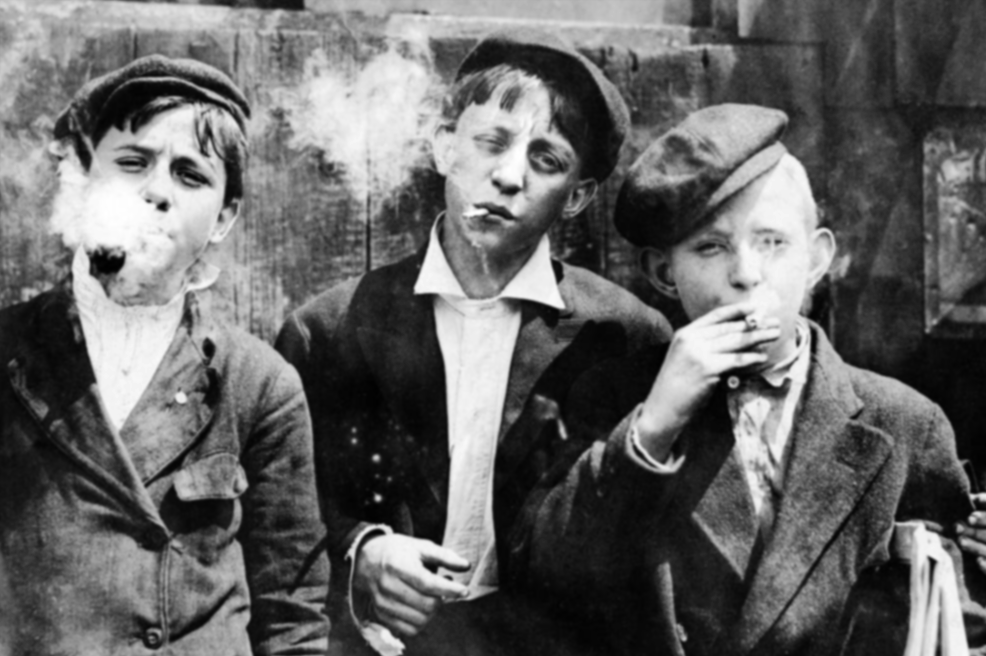
\includegraphics[width=0.85\textwidth]{images/result/task_2/Gaussian_fourier_5.png}
    \caption{Результат размытия по Гауссу при помощи преобразований Фурье при $N=5$}
    \label{fig:ga_f_5}
\end{figure}

\begin{figure}[ht!]
    \centering
    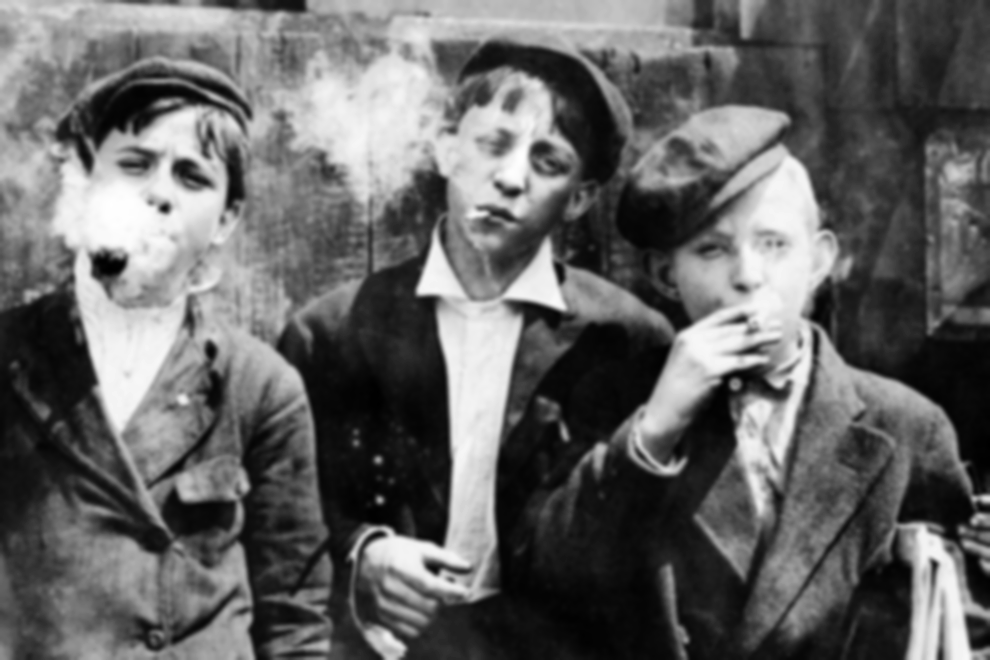
\includegraphics[width=0.95\textwidth]{images/result/task_2/Gaussian_9.png}
    \caption{Результат размытия по Гауссу при помощи свертки при $N=9$}
    \label{fig:ga_c_9}
\end{figure}

\begin{figure}[ht!]
    \centering
    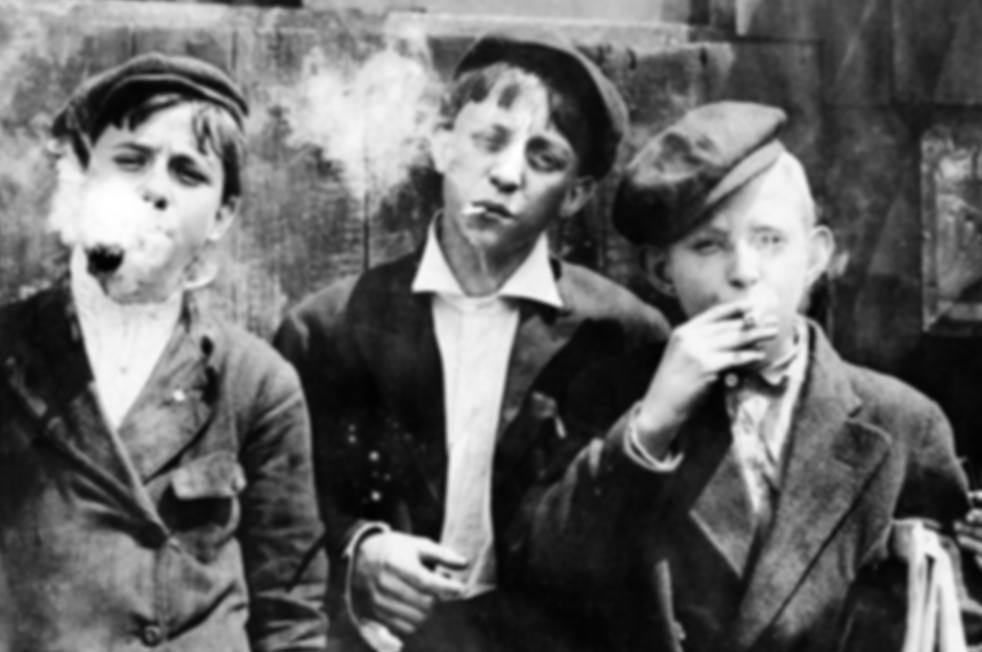
\includegraphics[width=0.95\textwidth]{images/result/task_2/Gaussian_fourier_9.png}
    \caption{Результат размытия по Гауссу при помощи преобразований Фурье при $N=9$}
    \label{fig:ga_f_9}
\end{figure}

\begin{figure}[ht!]
    \centering
    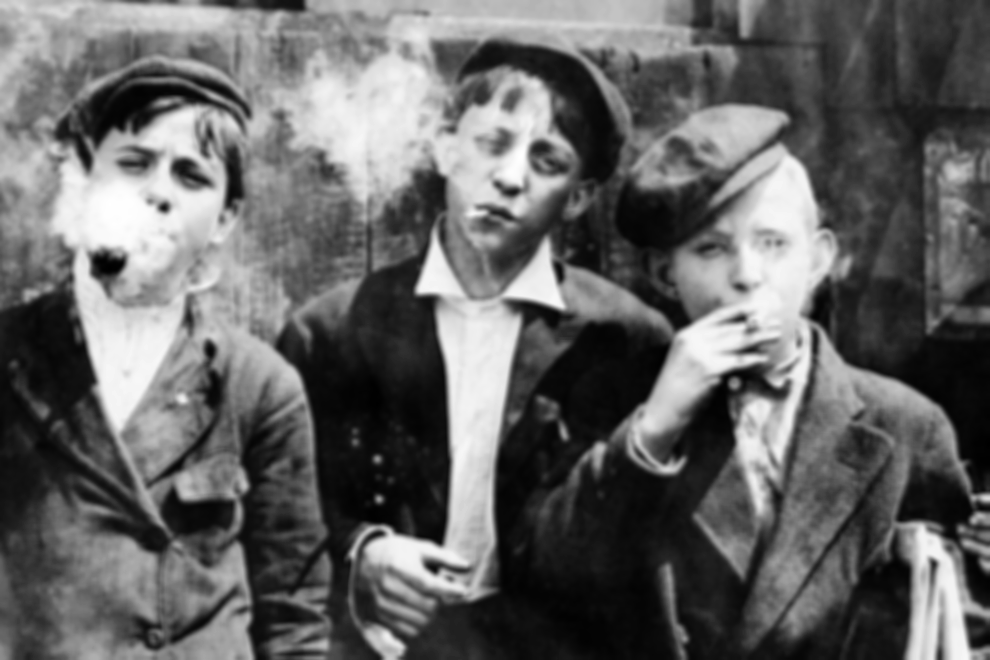
\includegraphics[width=0.95\textwidth]{images/result/task_2/Gaussian_11.png}
    \caption{Результат размытия по Гауссу при помощи свертки при $N=11$}
    \label{fig:ga_c_11}
\end{figure}

\begin{figure}[ht!]
    \centering
    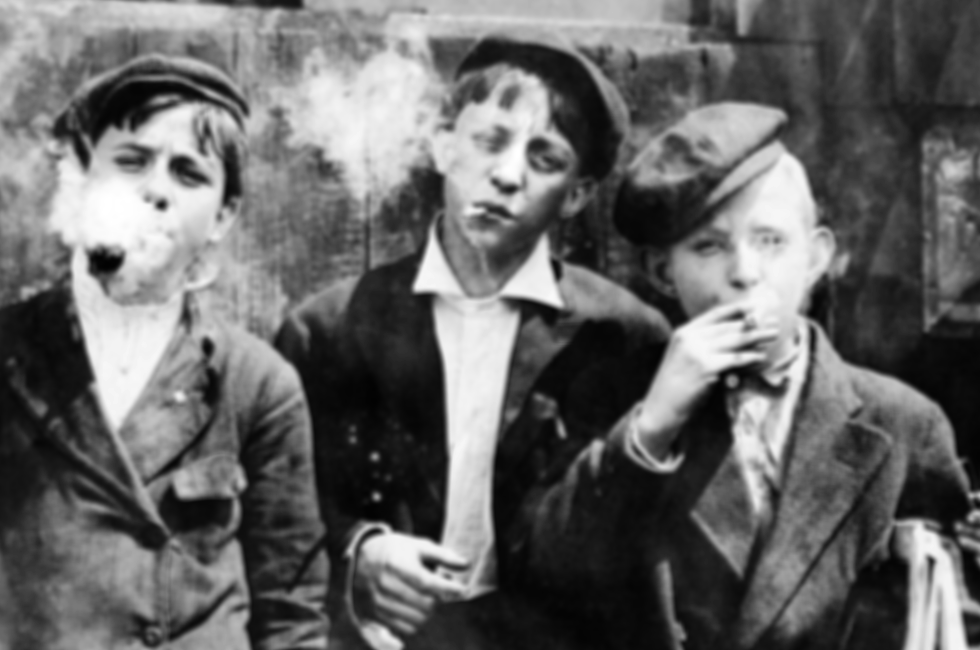
\includegraphics[width=0.95\textwidth]{images/result/task_2/Gaussian_fourier_11.png}
    \caption{Результат размытия по Гауссу при помощи преобразований Фурье при $N=11$}
    \label{fig:ga_f_11}
\end{figure}

Мы снова получили идентичные друг другу изображения. 

Результат гауссовского размытия получается более сглаженным в сравнении с блочным, будто на изображении лежит полупрозрачное стекло. Во втором случае возникает ощущение, что результат -- <<смазанное>> изображение более низкого качетсва.


\subsection{Увеличение резкости}

Для увеличения резкости воспользуемся матрицей

\begin{gather}
    K = \begin{pmatrix}
        0 & -1 & 0\\
        -1 & 5 & 1-\\
        0 & -1 & 0
    \end{pmatrix}  
\end{gather}

Получим результат применения этой матрицы на изображение посредством свёртки и Фурье-преобразований:

\begin{figure}[ht!]
    \centering
    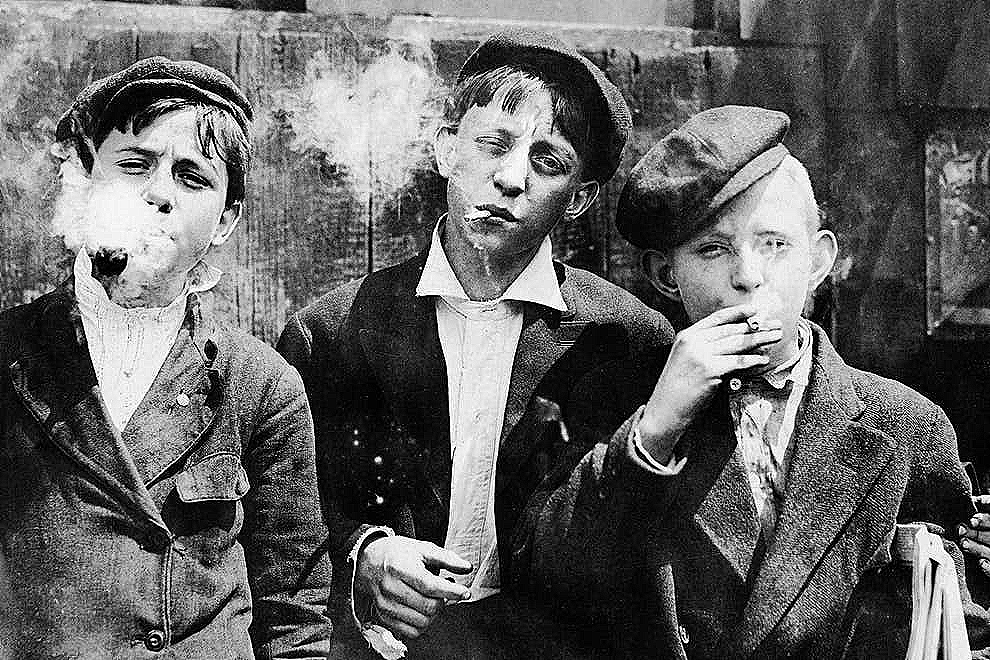
\includegraphics[width=0.95\textwidth]{images/result/task_3/Sharpened.png}
    \caption{Увеличение резкости изображения при помощи свертки}
    \label{fig:sh_c_5}
\end{figure}

\begin{figure}[ht!]
    \centering
    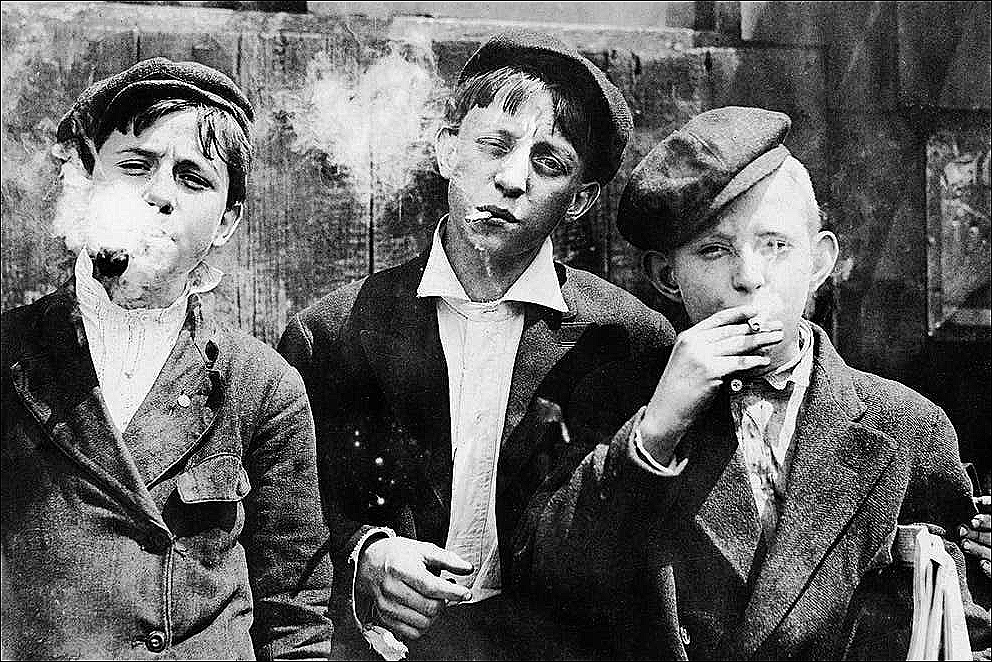
\includegraphics[width=0.95\textwidth]{images/result/task_3/Sharpened_fourier.png}
    \caption{Увеличение резкости изображения при помощи преобразований Фурье}
    \label{fig:sh_f_5}
\end{figure}
\clearpage
Полученные изображения идентичны друг другу. Единственное различие -- на изображении, полученном при использовании свертки, отсутствуют темные границы, так как свертка реализована при помощи функции \textit{filter2D()} из библиотеки \textit{OpenCV-Python}.
\FloatBarrier

\section{Выделение краёв}
Для последнего задания возьмем логотип немецкого производителя автомобилей -- \textbf{BMW}.

\begin{figure}[ht!]
    \centering
    
\includegraphics[width=0.5\textwidth]{images/source_images/task_4/bmw.jpeg}
    \caption{Логотип компании \textbf{BMW AG}}
    \label{fig:bmw}
\end{figure}
Для выделения контуров на изображении возьмём матрицу.
\begin{gather}
    K = \begin{pmatrix}
        -1 & -1 & -1\\
        -1 & 8 & 1-\\
        -1 & -1 & -1
    \end{pmatrix}  
\end{gather}

Применим её на изображение посредством свёртки и Фурье-преобразований:

\begin{figure}[ht!]
    \centering
    
\includegraphics[width=0.6\textwidth]{images/result/task_4/Edges.png}
    \caption{Контуры изображения, полученные при использовании свертки}
    \label{fig:ed_c}
\end{figure}

\begin{figure}[ht!]
    \centering
    
\includegraphics[width=0.6\textwidth]{images/result/task_4/Edges_fourier.png}
    \caption{Контуры изображения, полученные при использовании преобразований Фурье}
    \label{fig:ed_f}
\end{figure}

И снова мы получили одинаковые изображения (без учёта границы на изображении, полученном при использовании преобразований Фурье. Объяснение приведено в заключительном абзаце прошлого пункта).

Код программ для выполнения этой лабораторной работы и полученные изображения находятся в репозитории (\href{https://github.com/NikBrat/Lab_6_CM}{ссылка}).
\FloatBarrier % Content

\end{document}